\documentclass{article} 

\usepackage[utf8]{inputenc}
\usepackage{amssymb,amsmath}

\usepackage{graphicx}

\usepackage[top=3cm, bottom=3cm, left=3cm, right=3cm, includefoot]{geometry}

\usepackage{amsthm}
\theoremstyle{definition}
\newtheorem{definition}{Definition}

\begin{document}

\begin{definition}
\emph{Convex polytope} $\mathbf{S}$ is the set of all convex combinations of a finite point set $ \mathcal{S}$, i.e.
\begin{displaymath}
 \mathbf{S} :=
 \left\lbrace 
 v \in \mathbb{R}^n: v := \sum\limits_{i=1}^{\vert \mathcal{S} \vert} \alpha_i v_i; 
	\forall i = 1,\dots,\vert \mathcal{S} \vert: \alpha_i \geq 0, v_i \in \mathcal{S}, 
	\sum\limits_{i=1}^{\vert \mathcal{S} \vert} \alpha_i = 1 
 \right\rbrace.
\end{displaymath}
\end{definition}

Let us consider two convex polytopes $\mathbf{P}, \mathbf{Q}$ in $\mathbb{R}^d$ defined by the boundary point sets
\begin{displaymath}
 \begin{array}{rcll}
  \mathcal{P} & := & \lbrace p_1, \dots, p_{n_p} \rbrace \subset \mathbb{R}^d ~\mathrm{,} \\
  \mathcal{Q} & := & \lbrace q_1, \dots, q_{n_q} \rbrace \subset \mathbb{R}^d ~\mathrm{.}
 \end{array}
\end{displaymath}
The problem is to find the shortest distance between these two objects
\begin{equation}
 \label{eq:polytope_problem1}
 \min\limits_{p \in \mathcal{P}, q \in \mathcal{Q}} \Vert p - q \Vert ~\mathrm{.}
\end{equation}
Every interior point of the convex polytope can be expressed as a convex linear combination of given points in sets $\mathcal{P}$ and $\mathcal{Q}$
\begin{equation}
 \label{eq:polytope_linear_comb}
 \begin{array}{l}
  \forall p \in \mathbf{P} ~ \exists \alpha_1, \dots, \alpha_{n_p} \in \mathbb{R}: p = \sum\limits_{i = 1}^{n_p} \alpha_{i} p_i ~\mathcal{,} \\
	~~~~~~~~~~~~~~~~~~~~~~~ \mathrm{where} ~ \sum\limits_{i = 1}^{n_p} \alpha_i = 1 ~ \mathrm{and} ~ 0 \leq \alpha_i \leq 1 ~\forall i = 1,\dots,n_p ~\mathrm{,} \\
  \forall q \in \mathbf{Q} ~ \exists \beta_1, \dots, \beta_{n_q} \in \mathbb{R}: q = \sum\limits_{i = 1}^{n_q} \beta_{i} q_i ~\mathcal{,} \\
	~~~~~~~~~~~~~~~~~~~~~~~ \mathrm{where} ~ \sum\limits_{i = 1}^{n_q} \beta_i = 1 ~ \mathrm{and} ~ 0 \leq \beta_i \leq 1 ~\forall i = 1,\dots,n_q ~\mathrm{.}
 \end{array}
\end{equation} 
We denote
\begin{displaymath}
 \begin{array}{rcl}
  y & := & [\alpha_1, \dots, \alpha_{n_p}, \beta_1, \dots, \beta_{n_q}]^T \in \mathbb{R}^{n_p + n_q} ~\mathrm{,} \\
  C & := & [p_1, \dots, p_{n_p}, -q_1, \dots, -q_{n_q}] \in \mathbb{R}^{d, n_p + n_q} ~\mathrm{,} \\
  B & := & 
  \left[
   \begin{array}{cccccc}
    1 & \dots & 1 & 0 & \dots & 0 \\
    0 & \dots & 0 & 1 & \dots & 1 
   \end{array}   
  \right] \in \mathbb{R}^{2, n_p + n_q}  ~\mathrm{,} \\
  c & := & [1,1]^T \in \mathbb{R}^{2} \mathrm{.}
 \end{array}  
\end{displaymath}
Afterwards, the cost function can be reformulated
\begin{displaymath}
 \Vert p - q \Vert  = \left\Vert \sum\limits_{i = 1}^{n_p} \alpha_{i} p_i - \sum\limits_{i = 1}^{n_q} \beta_{i} q_i \right\Vert = \Vert Cy \Vert
\end{displaymath} 
and the feasible set conditions have the form
\begin{displaymath}
 By = c ~~~ \wedge ~~~ y \geq 0 ~\mathrm{.}
\end{displaymath}
After these notations, the problem \eqref{eq:polytope_problem1} can be reformulated as
\begin{equation}
 \label{eq:polytope_problem2}
 \begin{array}{rcl}
  \bar{y} & := & \arg \min\limits_{y \in \Omega_E \cap \Omega_I} y^T C^T C y ~\mathrm{,} \\
  \Omega_E & := & \left\lbrace y \in \mathbb{R}^{n_p + n_q}: By = c \right\rbrace ~\mathrm{,} \\
  \Omega_I & := & \left\lbrace y \in \mathbb{R}^{n_p + n_q}: y \geq 0 \right\rbrace ~\mathrm{.}
 \end{array}
\end{equation}
The next step consists of homogenization and orthogonalization. We introduce a substitution
\begin{equation}
 \label{eq:polytope_subs}
 x := y - y_{\mathrm{in}} ~~ \Rightarrow ~~ y = x + y_{\mathrm{in}} ~\mathrm{,}
\end{equation}
where $y_{in}$ is arbitrary point from $\Omega_E$. We can choose
\begin{displaymath}
 y_{\mathrm{in}} := \left[ \frac{1}{n_p}, \dots, \frac{1}{n_p}, \frac{1}{n_q}, \dots, \frac{1}{n_q} \right] \in \mathbb{R}^{n_p + n_q} ~\mathrm{.} 
\end{displaymath}
Afterwards, the cost function and conditions have the form
\begin{displaymath}
 \begin{array}{l}
  f(x) := \frac{1}{2} \Vert C(x + y_{\mathrm{in}}) \Vert^2 = \frac{1}{2} x^T \overbrace{C^T C}^{=: A} x + x^T \overbrace{C^T C y_{\mathrm{in}}}^{=: - b} + ~c, ~~~ c =: \frac{1}{2} y_{\mathrm{in}}^T C^T C y_{\mathrm{in}} = ~\mathrm{const.} ~\mathrm{,}\\
  B(x + y_{\mathrm{in}}) = Bx + B y_{\mathrm{in}} = Bx + c ~~~ \Rightarrow ~~~ ( By = c ~ \Leftrightarrow ~ Bx = 0) ~\mathrm{,} \\
  y \geq 0 ~~ \Leftrightarrow ~~ x \geq - y_{\mathrm{in}}  ~\mathrm{.}
 \end{array}
\end{displaymath}
Moreover, the matrix $B$ can be orthonormalized using simple process
\begin{displaymath}
 \hat{B} := 
 \left[
  \begin{array}{cc}
   \frac{1}{\sqrt{n_p}} & 0 \\
   0 & \frac{1}{\sqrt{n_q}}
  \end{array}
 \right] 
 B  ~\mathrm{.}
\end{displaymath}
We obtained QP with homogeneous orthogonal linear equality constraints and bound inequality constraints
\begin{equation}
 \label{eq:polytope_problem3}
 \begin{array}{rcl}
  \bar{x} & := & \arg \min\limits_{x \in \Omega_E \cap \Omega_I} \frac{1}{2} x^T A x - b^T x ~\mathrm{,} \\
  \Omega_E & := & \left\lbrace x \in \mathbb{R}^{n_p + n_q}: \hat{B}x = 0 \right\rbrace ~\mathrm{,} \\
  \Omega_I & := & \left\lbrace x \in \mathbb{R}^{n_p + n_q}: x \geq -y_{\mathrm{in}} \right\rbrace ~\mathrm{.}
 \end{array}
\end{equation}
After solving this problem, the original solution can be obtained using back substitution \eqref{eq:polytope_subs} to obtain $y$, i.e. the coeficients of linear combinations \eqref{eq:polytope_linear_comb} of the nearest points from each polytope.

%\newpage

\paragraph{Numerical example}

We consider two circles discretized by parameter $m \geq 3$, whose boundary points are defined by $P, Q \in \mathbb{R}^{2,m}$
with columns
\begin{displaymath}
 P_{\ast,i} = 
 \left[
  \begin{array}{c}
   \cos (2i\pi / m ) - 2  \\
   \sin (2i\pi / m ) 
  \end{array}
 \right]
 , ~~~
 Q_{\ast,i} = 
 \left[
  \begin{array}{c}
   \cos (\pi - 2i\pi / m ) + 2 \\
   \sin (\pi - 2i\pi / m ) 
  \end{array}
 \right], ~~~
 i = 0,\dots,m-1 ~\mathrm{.} 
\end{displaymath}
Examples for $m = 5$ and $m=7$ can be found in Fig. \ref{fig:polytope1}.

\begin{figure}[h!]
\begin{center}
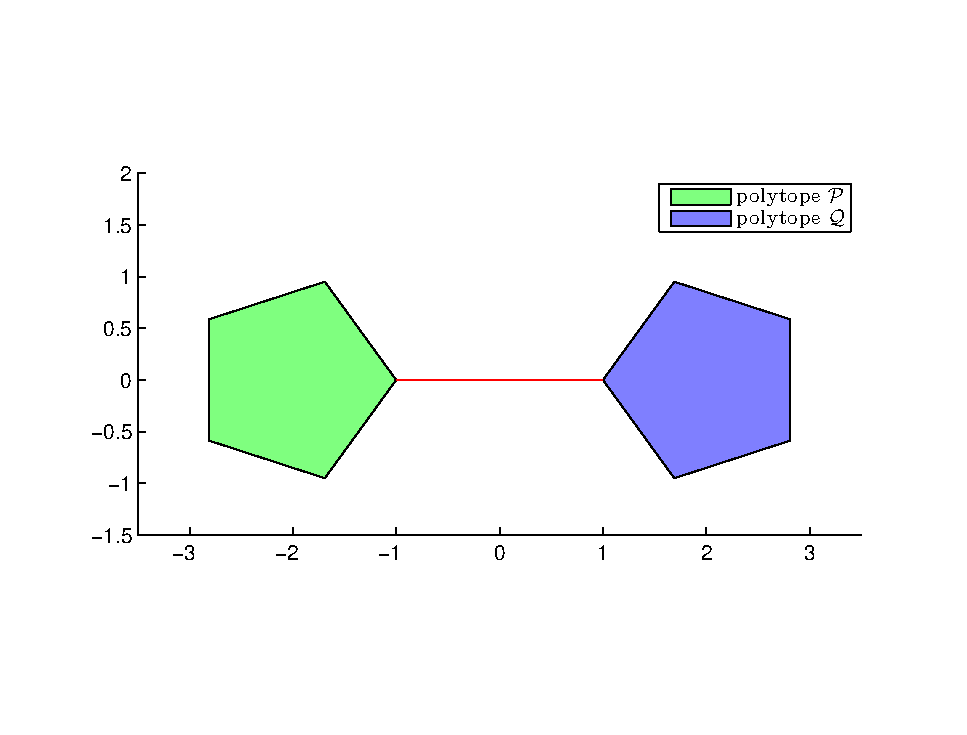
\includegraphics[width=0.45\textwidth]{polytope_n5.eps}
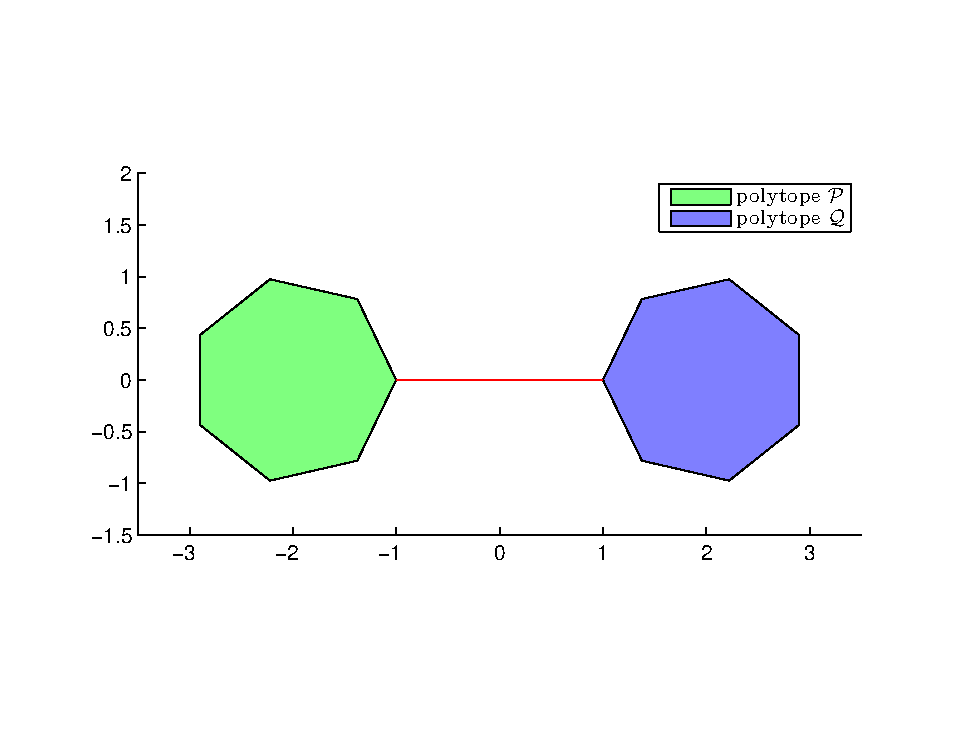
\includegraphics[width=0.45\textwidth]{polytope_n7.eps}
\caption[Polytope distance: testing benchmark]{Testing benchmark for polytopes distance with discretization parameter $m = 5$ \emph{(left)} and $m = 7$ \emph{(right)}.}
\label{fig:polytope1}
\end{center}
\end{figure}

The solution of the problem for any $m$ is given by
\begin{displaymath}
 \bar{y} =
 \left[
  \alpha_1, \dots, \alpha_m, \beta_1, \dots, \beta_m
 \right]^T = 
 [\underbrace{1 , 0, \dots, 0}_{\in \mathbb{R}^m}, \underbrace{1 , 0, \dots, 0}_{\in \mathbb{R}^m}]^T ~\mathrm{.}  
\end{displaymath}

In this problem, we can directly compute the regular condition number of Hessian matrix 
\begin{displaymath}
 \kappa (A) = \kappa (C^T C) = \kappa (CC^T) = \kappa
 \left( \left[
  \begin{array}{cc}
   \sum\limits_{i = 1}^{n_p} P_{i,1}^2 + \sum\limits_{i = 1}^{n_q} Q_{i,1}^2 & \sum\limits_{i = 1}^{n_p} P_{i,1} P_{i,2} + \sum\limits_{i = 1}^{n_q} Q_{i,1} Q_{i,2} \\
   \sum\limits_{i = 1}^{n_p} P_{i,2} P_{i,1} + \sum\limits_{i = 1}^{n_q} Q_{i,2} Q_{i,1} & \sum\limits_{i = 1}^{n_p} P_{i,2}^2 + \sum\limits_{i = 1}^{n_q} Q_{i,2}^2
  \end{array}
 \right] \right) ~\mathrm{.}
\end{displaymath}
Moreover, it holds
\begin{displaymath}
 \begin{array}{rcl}
 \sum\limits_{i = 1}^{n_p} P_{i,2} P_{i,1} + \sum\limits_{i = 1}^{n_q} Q_{i,2} Q_{i,1} & = &
	\sum\limits_{i = 0}^{m-1} 
		\left( \cos \left( \frac{2i\pi}{m} \right) - 2 \right)
		\sin \left( \frac{2i\pi}{m} \right) \\
  & & ~~~~~ + 
 \sum\limits_{i = 0}^{m-1} 
  \left( \cos \left( \pi - \frac{2i\pi}{m} \right) + 2 \right)
  \sin \left( \pi - \frac{2i\pi}{m} \right)
 = 0~\mathrm{,}
 \end{array} 
\end{displaymath}
so
\begin{displaymath}
 \kappa (A) = \kappa
 \left( \left[
  \begin{array}{cc}
   \sum\limits_{i = 1}^{n_p} P_{i,1}^2 + \sum\limits_{i = 1}^{n_q} Q_{i,1}^2 & 0 \\
   0 & \sum\limits_{i = 1}^{n_p} P_{i,2}^2 + \sum\limits_{i = 1}^{n_q} Q_{i,2}^2
  \end{array}
 \right] \right) ~\mathrm{.}
\end{displaymath}
Afterwards, the condition number can be expressed
\begin{displaymath}
\kappa (A) = \frac{\sum\limits_{i = 1}^{n_p} P_{i,1}^2 + \sum\limits_{i = 1}^{n_q} Q_{i,1}^2}{\sum\limits_{i = 1}^{n_p} P_{i,2}^2 + \sum\limits_{i = 1}^{n_q} Q_{i,2}^2} =
\frac{\sum\limits_{i=0}^{m-1} \left( \cos \left( \frac{2i\pi}{m} \right) - 2 \right)^2}{\sum\limits_{i=0}^{m-1} \sin^2 \left( \frac{2i\pi}{m} \right)} ~~~~ \forall m \geq 3 ~\mathrm{.}
\end{displaymath}

\noindent Let us consider $\alpha \in \mathbb{R}$ and let us present a complex number $z \in \mathbb{C}$ by prescription
\begin{displaymath}
 z := \cos \alpha + \mathbf{i} \sin \alpha ~\mathrm{,}
\end{displaymath}
where $\mathbf{i}$ is imaginary unit. Then by De Moivre's formula we can write
\begin{displaymath}
 \sum\limits_{i=0}^{m-1} \left( \cos ( i\alpha) + \mathbf{i} \sin ( i \alpha) \right) =
 \sum\limits_{i=0}^{m-1} z^i =
 \frac{z^m - 1}{z - 1} =
 \frac{\cos (m\alpha) + \mathbf{i} \sin (m\alpha) - 1}{z-1} ~\mathrm{.}
\end{displaymath}
If we choose specific $\alpha$ in previous equality, we obtain next
\begin{equation}
 \label{eq:polytope_ne_pom}
  \begin{array}{ccccc}
   \alpha := \frac{2 \pi}{m}& ~ \Rightarrow ~ & \sum\limits_{i=0}^{m-1} \left( \cos \left( \frac{2i\pi}{m} \right) + \mathbf{i} \sin \left( \frac{2i\pi}{m} \right) \right) = 0 & ~ \Rightarrow ~ & \sum\limits_{i=0}^{m-1} \cos \left( \frac{2i\pi}{m} \right) = 0\mathrm{,}\\ 
   \alpha := \frac{4 \pi}{m}& ~ \Rightarrow ~ & \sum\limits_{i=0}^{m-1} \left( \cos \left( \frac{4i\pi}{m} \right) + \mathbf{i} \sin \left( \frac{4i\pi}{m} \right) \right) = 0 & ~ \Rightarrow ~ & \sum\limits_{i=0}^{m-1} \cos \left( \frac{4i\pi}{m} \right) = 0\mathrm{.}
  \end{array}
\end{equation}
Now, we return back to regular condition number and $\forall m \geq 3$ we can write (using \eqref{eq:polytope_ne_pom})
\begin{displaymath} 
 \begin{array}{rl}
   \kappa (A) = & \frac{\sum\limits_{i=0}^{m-1} \left( \cos \left( \frac{2i\pi}{m} \right) - 2 \right)^2}{\sum\limits_{i=0}^{m-1} \sin^2 \left( \frac{2i\pi}{m} \right)} 
= \frac{\sum\limits_{i=0}^{m-1} \cos^2 \left( \frac{2i\pi}{m} \right) - 4 \cos \left( \frac{2i\pi}{m} \right) + 4}{\sum\limits_{i=0}^{m-1} \sin^2 \left( \frac{2i\pi}{m} \right)} \\
 & = \frac{\sum\limits_{i=0}^{m-1} \left( \frac{1 + \cos \left( \frac{4i\pi}{m} \right)}{2} - 4 \cos \left( \frac{2i\pi}{m} \right) + 4 \right)}{\sum\limits_{i=0}^{m-1} 
  \frac{1 - \cos \left( \frac{4i\pi}{m} \right)}{2}} 
 =  \frac{ \frac{1}{2} \sum\limits_{i=0}^{m-1} \cos \left( \frac{4i\pi}{m} \right) - 4 \sum\limits_{i=0}^{m-1} \cos \left( \frac{2i\pi}{m} \right) + \sum\limits_{i=0}^{m-1} \frac{9}{2}   }{-\frac{1}{2}\sum\limits_{i=0}^{m-1} \cos \left( \frac{4i\pi}{m} \right) + \sum\limits_{i=0}^{m-1} \frac{1}{2} } = 9 ~\mathrm{.}
 \end{array} 
\end{displaymath}


\end{document}

